\documentclass[11pt]{article}
\usepackage[utf8]{inputenc}
\usepackage[T2A]{fontenc}
\usepackage[english, russian]{babel}
\usepackage{amsmath,amssymb,amsfonts,tikz}
\usepackage{graphicx}
\usepackage{booktabs}
\usepackage{hyperref}
\usepackage[most]{tcolorbox}
\usepackage{tabularx}
\usepackage{float}
\usepackage[style=verbose-ibid,backend=biber]{biblatex}
\addbibresource{references.bib}
\usepackage[margin=2.5cm]{geometry}
\usepackage{fancyhdr}
\usepackage{xcolor}
\definecolor{blockblue}{RGB}{204,229,255}
\definecolor{blockred}{RGB}{255,229,204}

\pagestyle{fancy}
\fancyhf{}
\fancyhead[L]{Инструменты разделения редких ресурсов}
\fancyhead[R]{\thepage}
\renewcommand{\headrulewidth}{0.4pt}

\title{Инструменты разделения редких и\\ неравномерно распределённых ресурсов}
\author{Мещеряков Вадим, Иванова Дарья, Мишаков Андрей, Петрунников Тимур}
\date{\today}

\begin{document}
\maketitle

% ================= 1. ВВЕДЕНИЕ =================
\section{Введение: почему это не про «рынок или государство»}

Население хочет \textbf{тепло}, а не нефть. Спрос на нефть — производный: чтобы получить единицу блага $i$ (перевозка, свет, отопление, продукция промышленности), нужно $a_i$ единиц нефти, поэтому
\[
D_{oil}(p) = \sum_{i} a_i\, D_i(p_i),
\]
где $a_i$ — расход нефти на единицу блага $i$, а $D_i(p_i)$ — спрос на само благо $i$. Совокупный спрос на нефть складывается из этих производных спросов, взвешенных технологическими коэффициентами $a_i$.

\textbf{Конкуренция} за ресурс идёт не на уровне домохозяйств, а на уровне:
\begin{itemize}
\item фирм (НПЗ, трейдеры, агроэкспорт),
\item государств (права на добычу, концессии, трансграничные воды).
\end{itemize}

Отсюда \textbf{ложная развилка}: «рынок или государство». Инструментарий шире — и сегодня мы инвентаризируем его как инженеры: без оценок, через параметры.

% ================= 2. ТРИ ОСИ =================
\section{Три оси — не путать}

Три понятия, которые в бытовой речи сливаются, — \textbf{ограниченность}, \textbf{редкость}, \textbf{неравномерность} — имеют разную природу и требуют разных инструментов.

\subsection{Ограниченность (flow / stock)}
Физический факт: \emph{потоковый} ресурс $\dot{Q} \le R$, \emph{запасовый} — $Q_{total} \le S$.

\textbf{Индикатор:} горизонт исчерпания $R/Q$ (отношение запаса к текущей добыче, \emph{Reserve-to-Production}, $R/P$).
\[
R/P = \frac{S}{\dot{Q}}
\]
Порог $R/P < 20$ лет обычно читается как сигнал тревоги, но сам по себе не означает редкость: он говорит только о горизонте физического исчерпания при текущем темпе добычи, а не об экономическом дефиците. Пример: у фосфатных пород по разным оценкам конца 1970-х--1980-х годов $R/P$ оценивался в районе 100--400 лет в зависимости от того, какие месторождения относить к разведанным запасам; более поздние, более консервативные по определению запасов оценки называют существенно более низкий горизонт. Сам факт большого разброса оценок — хороший повод показать аудитории, что $R/P$ — грубый и нестабильный индикатор, сильно зависящий от определения «запасов».

\textbf{Важно:} если $R/Q \to \infty$ (поток), но $S(0) \le 0$ (нет избыточного спроса при нулевой цене) — \emph{инструменты распределения не нужны}.

\subsubsection{Индикаторы водного стресса}
Здесь стоит различать два разных, часто путаемых индекса.

\textbf{Индекс Фалькенмарка} (подушевая доступность) \cite{falkenmark1989}:
\[
W = \frac{\text{Возобновляемые водные ресурсы в год}}{\text{Население}}\quad [\text{м}^3/\text{чел}/\text{год}]
\]
Общепринятые пороги: $W>1700$ — нет стресса, $1000<W<1700$ — умеренный стресс, $W<1000$ — дефицит, $W<500$ — абсолютный дефицит.

\textbf{Коэффициент критичности (Raskin et al.)} \cite{raskin1997watersupply} — отношение изъятий к доступному объёму:
\[
WTA = \frac{\text{Total withdrawals}}{\text{Total renewable supply}}
\]
Пороги: $WTA<0.1$ — нормальный режим, $0.1<WTA<0.2$ — умеренный стресс, $0.2<WTA<0.4$ — высокий стресс, $WTA>0.4$ — хронический острый стресс.

Это два разных по конструкции индекса (подушевой запас против доли изъятия), их не стоит смешивать в один «WSI» с одними и теми же порогами.

\subsection{Редкость (scarcity)}
Экономическое понятие: $S = D(0) - Q$ — избыточный спрос при нулевой цене.

\subsubsection{Эластичность предложения}
\[
\eta = \frac{\Delta Q/Q}{\Delta p/p}
\]
$\eta \to 0$ — вертикальная кривая предложения (редкость не снимается ценой). Пример: нефть в коротком периоде — низкая эластичность предложения (порядка нескольких сотых), донорские органы — эластичность практически нулевая, поскольку легальное предложение не реагирует на цену вовсе.

Параметры, определяющие редкость:
\begin{itemize}
\item эластичность предложения (если $\eta \to \infty$ — редкость не растёт при росте спроса),
\item наличие положительной экономической ренты в цене,
\item отношение запасы/добыча (грубый индикатор, см.\ выше).
\end{itemize}

\textbf{Пример:} воздух в чистом месте — $S(0) \le 0$ — не редок; воздух в мегаполисе — $S(0) > 0$ — редок.

\subsection{Неравномерность}
\textbf{Не то же, что редкость.} Это про «где ресурс находится и у кого права».

\subsubsection{Кривая Лоренца}
Пусть $F(x)$ — функция распределения доходов или прав, $F^{-1}(p)$ — квантильная функция, $\mu$ — среднее значение. Кривая Лоренца:
\[
L(p) = \frac{1}{\mu}\int_0^p F^{-1}(t)\,dt,\qquad p\in[0,1].
\]
Свойства: $L(0)=0$, $L(1)=1$, $L(p)\le p$.

\subsubsection{Индекс Джини}
\[
G = 1 - 2\int_0^1 L(p)\,dp = \frac{\sum_{i=1}^n\sum_{j=1}^n |x_i-x_j|}{2n^2\mu}.
\]
\textbf{Корректная интерпретация:} $G$ — это средняя абсолютная разница между всеми парами значений в выборке, отнесённая к удвоенному среднему. Ориентировочные пороги: $G<0.3$ — сравнительно равномерное распределение, $0.3<G<0.5$ — умеренное неравенство, $G>0.5$ — острое неравенство (границы условны и зависят от контекста — дохода, земли, прав на ресурс).

\subsubsection{Коэффициент вариации}
\[
CV = \frac{\sigma}{\mu}.
\]
Ориентировочные пороги: $CV<0.3$ — слабая вариация, $0.3<CV<0.6$ — средняя, $CV>0.6$ — сильная. В отличие от индекса Джини, $CV$ более чувствителен к выбросам в хвосте распределения.

\subsubsection{Индекс Херфиндаля--Хиршмана (HHI)}
Пусть $s_i$ — доля $i$-го держателя прав в процентах, $\sum s_i = 100$. Тогда
\[
HHI = \sum_{i=1}^N s_i^2 \in [0,\,10000].
\]
HHI изначально применяется в антимонопольном анализе товарных рынков; мы заимствуем его здесь как удобный измеритель институциональной концентрации прав. По действующим Merger Guidelines 2023 (US DOJ/FTC) \cite{ftc_doj_2023merger} ориентир таков: $HHI<1000$ — низкая концентрация, $1000<HHI<1800$ — умеренная, $HHI>1800$ — высокая концентрация. Эти пороги калиброваны для рынков товаров, а не для держателей водных или иных ресурсных прав, — перенос на права на ресурсы носит иллюстративный, а не строго обоснованный характер, и численный пример по Чили здесь не приводится за отсутствием надёжного источника.

Три параметра разной природы стоят за неравномерностью:
\begin{enumerate}
\item \textbf{Геологическая концентрация} — доля мировых запасов в топ-$N$ странах (кобальт — ДР Конго, литий — «литиевый треугольник»).
\item \textbf{Институциональная концентрация} — концентрация прав (HHI по держателям лицензий). Именно об этой оси идёт речь у Перкинса (см.\ раздел~\ref{sec:perkins}): не «нефти нет у населения», а «права на нефть не у населения».
\item \textbf{Неравномерность доступа по покупательной способности} — даже при глобально достаточном объёме. Сен: голод — не от нехватки еды, а от краха entitlement.
\end{enumerate}

\subsection{Ограниченность vs Редкость — когда они расходятся}
\begin{itemize}
\item \textbf{Пастбище:} трава растёт с темпом $R$. Пока $R \ge$ изъятия — система устойчива.
\item \textbf{То же пастбище:} если $D(0) > R$, даже при устойчивом $R$ — дефицит при нулевой цене.
\item \textbf{Воздух:} поток не ограничен, но $S(0) \le 0$ — не редок.
\end{itemize}
\textbf{Вывод:} ограниченность — необходимое, но не достаточное условие редкости.

% ================= 3. МАТРИЦА =================
\section{Матрица исключаемость / соперничество}

\begin{figure}[h]
\centering
\begin{tikzpicture}[scale=0.9]
\draw[->] (0,0) -- (6,0) node[right] {Исключаемость};
\draw[->] (0,0) -- (0,5) node[above] {Соперничество};
\draw[thick] (0,0) rectangle (3,3) node[midway] {\shortstack{Общественные блага\\(оборона, знание)}};
\draw[thick] (3,0) rectangle (6,3) node[midway] {\shortstack{Клубные\\(спутник, платный доступ)}};
\draw[thick] (0,3) rectangle (3,6) node[midway] {\shortstack{Commons / открытый\\доступ (пастбище, рыба)}};
\draw[thick] (3,3) rectangle (6,6) node[midway] {\shortstack{Частные\\(нефть, зерно)}};
\node at (1.5,-0.6) {\footnotesize низкая};
\node at (4.5,-0.6) {\footnotesize высокая};
\end{tikzpicture}
\caption{Четыре типа благ по соперничеству и исключаемости}
\end{figure}

Верхний левый квадрант (неисключаемый + соперничающий) — это и есть зона классической «трагедии общин»; при введении правил сообщества она превращается в устойчивые commons, без правил — деградирует в открытый доступ. Это один и тот же тип блага, разница — в режиме собственности, который на него наложен.

\textbf{Ключевой вывод:} сам по себе факт, что ресурс «общий» (неисключаемый и соперничающий), ещё не означает трагедии — нужен \textbf{режим собственности} \cite{ostrom1990governing}.

% ================= 4. ИНСТРУМЕНТАРИЙ =================
\section{Инструментарий — три блока}

\subsection{Блок 1. Режимы собственности}
\begin{itemize}
\item \textbf{Частная} — спецификация прав, можно продать (ITQ в Исландии).
\item \textbf{Государственная} — концессии, лицензии, государственная собственность на недра.
\item \textbf{Общая (commons)} — правила сообщества, исключение чужих (huertas Валенсии, японские сатояма).
\item \textbf{Открытый доступ} — \emph{не является институтом}, это отсутствие режима.
\end{itemize}
\textbf{Важно:} реальные системы — гибриды. Рыболовные квоты — государственная собственность + временное частное право + перепродажа.

\subsection{Блок 2. Механизмы распределения}
\textbf{Рыночные:}
\begin{itemize}
\item аукцион (английский, голландский, Vickrey — доминирующая стратегия сообщать истинную оценку) \cite{vickrey1961counter},
\item переуступаемые квоты (ITQ, cap-and-trade).
\end{itemize}
\textbf{Административные:}
\begin{itemize}
\item нормирование (карточная система, водный паёк при дефиците),
\item очередь (\emph{first-come-first-served}),
\item лотерея (грин-карта, разрешения на охоту),
\item административное распределение по баллу (UNOS — совместимость + срочность + ожидание).
\end{itemize}
\textbf{Гибрид:} ITQ — государство устанавливает $\sum E_i = E_{cap}$, затем права торгуются.

\subsection{Блок 3. Механизмы ограничения}
Два подхода — Пигу vs Коуз.

\textbf{Пигу:} обложить использование налогом = предельный внешний эффект.

\textbf{Коуз:} чёткие права + рынок (cap-and-trade).

\textbf{Command-and-control:}
\begin{itemize}
\item технологические стандарты,
\item абсолютные лимиты (квоты вылова),
\item зонирование,
\item концессии с условиями,
\item ротация (севооборот, пастбища).
\end{itemize}

\textbf{Правила самоуправления (Остром)} \cite{ostrom1990governing} — восемь принципов устойчивых commons:
\begin{enumerate}
\item чётко определённые границы ресурса и круга пользователей;
\item соответствие правил присвоения и обеспечения местным условиям;
\item коллективный выбор правил самими пользователями;
\item мониторинг, подотчётный самим пользователям;
\item градуированные санкции за нарушения;
\item доступные и недорогие механизмы разрешения конфликтов;
\item минимальное признание права сообщества на самоорганизацию со стороны государства;
\item вложенность институтов при использовании ресурса, охватывающего несколько уровней.
\end{enumerate}

\begin{table}[H]
\centering
\begin{tabular}{@{}lccc@{}}
\toprule
\textbf{Благо / Инструмент} & \textbf{Рынок} & \textbf{Община / Квота} & \textbf{VCG / Гейл--Шепли} \\
\midrule
Нефть (частное)            & \checkmark & -- & -- \\
Спутник (клубное)          & \checkmark & -- & -- \\
Оборона (общественное)     & -- & \checkmark (налог) & \checkmark (опрос) \\
Пастбище (commons)         & \checkmark (ITQ) & \checkmark (Остром) & -- \\
Вода (Чили)                & \checkmark (широкий рынок) & -- & -- \\
Вода (Австралия)           & -- & \checkmark (cap) & -- \\
Органы (UNOS)              & -- & -- & \checkmark (балл / MELD) \\
\bottomrule
\end{tabular}
\caption{Какой инструмент используется для какого блага}
\end{table}

% ================= 5. КЕЙС: ВОДА =================
\section{Кейс: вода — Чили (1981) vs Австралия (Murray--Darling)}

\subsection{Чили}
Водный кодекс 1981 года отделил права на воду от земли и сделал их торгуемыми, бессрочными правами \cite{bauer1998chile}. На уровне бассейнов долгое время не было обязательного экологического потолка изъятий. Результат — концентрация прав в руках крупного агроэкспорта и заметное сокращение стока в отдельных бассейнах в засушливые годы, в том числе в бассейне реки Петорка \cite{budds2008chapter}.

\textbf{Важное уточнение:} в 2022 году вступила в силу реформа (Закон №21.435): новые права теперь выдаются на срок до 30 лет вместо бессрочных, закреплён приоритет водоснабжения населения и введено изъятие прав за неиспользование \cite{chile2022reform}. Классическое сравнение «Чили vs Австралия» относится прежде всего к режиму 1981--2022 годов; текущая система — уже гибрид рынка и государственного регулирования.

\subsection{Австралия}
$\bar{Q}$ — экологически устойчивый объём изъятий бассейна, $q_i = e_i \cdot \bar{Q}/\sum e_i$ — доля пользователя $i$ в этом потолке \cite{grafton2014water}. Во время «Тысячелетней засухи» (примерно 1997--2009) объём водопользования в бассейне Мюррей--Дарлинг упал на 33--67\% в зависимости от года и подрегиона; номинальная стоимость орошаемого производства при этом снизилась заметно слабее — по разным оценкам на 14--20\% \cite{kirby2014drought}, а суммарный эффект на ВВП сельского хозяйства региона оценивается порядка нескольких процентов регионального продукта (около 0.75\% ВВП всей Австралии за период засухи). Смягчить удар помогли рост товарных цен и активная торговля временными аллокациями.

\subsection{Формальная разница}
\noindent
\begin{minipage}[t]{0.45\textwidth}
\textbf{Чили (до 2022 г.):}
\[
q_i \ge 0,\quad \sum q_i \text{ не ограничена жёстким потолком}
\]
Цена стремится к предельным издержкам добычи/подъёма воды, а не к её экологической ценности.
\end{minipage}\hfill
\begin{minipage}[t]{0.45\textwidth}
\textbf{Австралия:}
\[
\bar{Q} = \sum q_i,\quad q_i = e_i \cdot \frac{\bar{Q}}{\sum e_i}
\]
Торгуется \emph{доля} потолка. В засуху $\bar{Q}$ падает — цена аллокации растёт, но суммарный объём остаётся $\le \bar{Q}$.
\end{minipage}

\textbf{Одна и та же идея (торгуемые права) $\Rightarrow$ разные результаты — в зависимости от того, есть ли жёсткий экологический потолок.}

% ================= 6. ВАЙЦМАН =================
\section{Правило Вайцмана (1974): цена vs количество}

\subsection{Модель}
Регулятор выбирает между:
\begin{itemize}
\item \textbf{ценой} (налог) — $p$ фиксирована, $q$ подстраивается,
\item \textbf{количеством} (квота) — $\bar{q}$ фиксирована, $p$ подстраивается.
\end{itemize}

При линейных предельной выгоде и предельных издержках и неопределённости в положении кривой $MC$, для квадратичных функций потерь \cite{weitzman1974prices}:
\begin{equation}\label{eq:weitzman}
\frac{L_{\text{price}}}{L_{\text{quota}}} = \left( \frac{e}{f} \right)^2,
\end{equation}
где $e$ — наклон $MB$, $f$ — наклон $MC$.

\subsection{Интерпретация}
\begin{itemize}
\item $e < f$ (MB более пологая, чем MC) $\Rightarrow$ ошибка в цене обходится дешевле ошибки в количестве $\Rightarrow$ \textbf{налог} предпочтительнее.
\item $e > f$ (MB более крутая, чем MC) $\Rightarrow$ \textbf{квота} предпочтительнее.
\item При «толстых хвостах» распределения ущерба, то есть при риске катастрофического исхода вблизи порога, соображение из \eqref{eq:weitzman} перестаёт быть решающим и практический аргумент смещается в пользу \textbf{квоты} как более надёжного ограничителя объёма \cite{weitzman2009tails}.
\end{itemize}

\subsection{Иллюстрация: углерод}
Для CO$_2$ часто утверждают, что на горизонте одного года предельный ущерб (MB избегания) относительно пологий по сравнению с предельными издержками резкой декарбонизации (MC), что по правилу Вайцмана говорит в пользу налога, а не жёсткой квоты на конкретный год. Ориентир по уровню цены: по расчётам модели DICE-2016R социальная цена углерода оценивалась примерно в \$31 за тонну CO$_2$ в ценах 2010 года на 2015 год, с ростом около 3\% в год \cite{nordhaus2017scc}. Это одна из многих оценок среди широкого разброса в литературе, а не единственно верное число.

\begin{figure}[h]
\centering
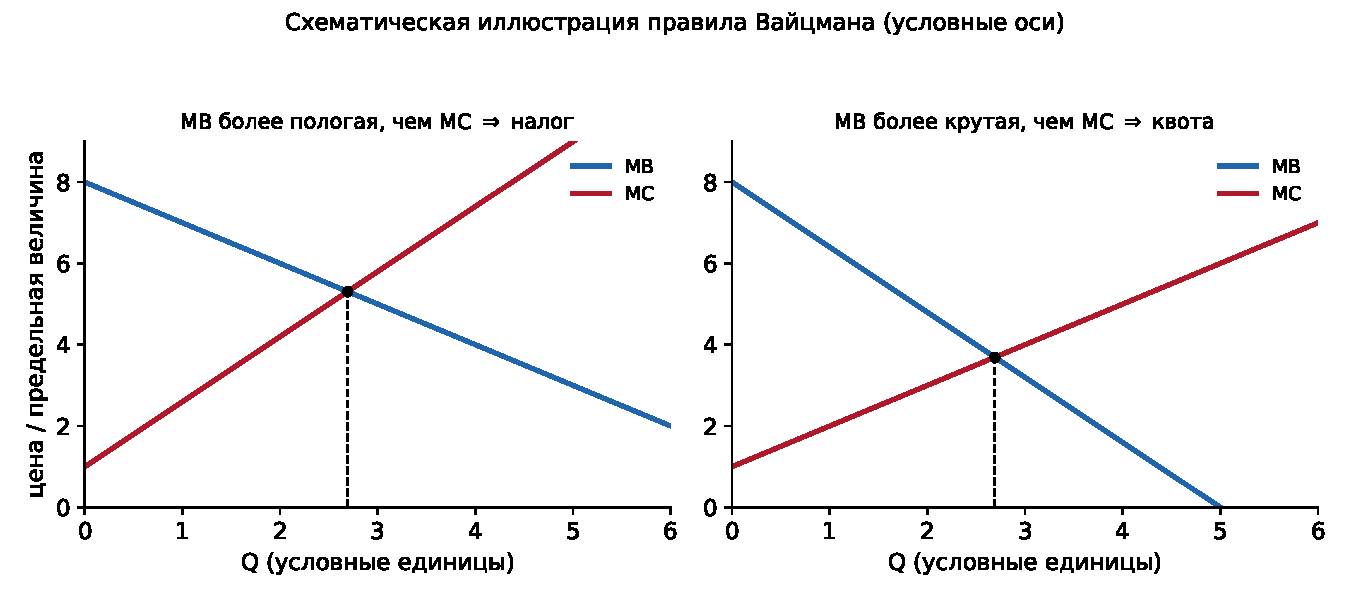
\includegraphics[width=0.75\linewidth]{weitzman_schematic.pdf}
\caption{Схематическая иллюстрация правила Вайцмана: слева MB более пологая, чем MC — предпочтителен налог; справа MB более крутая — предпочтительна квота. Значения на осях условны и не воспроизводят конкретную эмпирическую модель.}
\end{figure}

% ================= 7. VCG И ГЕЙЛ-ШЕПЛИ =================
\section{Формальные механизмы: VCG и Гейл--Шепли}
\label{sec:vcg_gs}

\subsection{VCG — платежи за общественное благо}
\begin{equation}\label{eq:vcg}
x^*(\theta) = \arg\max_{x\in X} \sum_{i=1}^n v_i(x,\theta_i), \qquad
p_i(\theta) = \max_{x\in X} \sum_{j\neq i} v_j(x,\theta_j) - \sum_{j\neq i} v_j(x^*,\theta_j)
\end{equation}
Правило Кларка: каждый участник платит ровно тот внешний эффект, который его присутствие накладывает на остальных.

\textbf{Пример:} три города A, B, C рассматривают дорогу A--B стоимостью 12; выгоды: $v_A=8$, $v_B=6$, $v_C=0$. Строить эффективно, так как $8+6+0=14>12$. Без города A выгода оставшихся от постройки была бы $6-12<0$, то есть без A дорогу строить не стали бы; платёж A по правилу Кларка равен внешнему эффекту, который A накладывает на остальных: $p_A = 0 - (6-12) = 6$. Аналогично без B выгода оставшихся $8-12<0$, дорогу не строят; $p_B = 0-(8-12)=4$. Город C, чья выгода равна нулю, ничего не платит и не меняет решение ни для кого: $p_C=0$. Суммарные платежи $6+4+0=10<12$ — типичный для механизма Кларка \emph{дефицит бюджета}: VCG гарантирует эффективность и правдивость, но не балансирует бюджет.

\subsection{Гейл--Шепли — стабильное паросочетание}
\begin{itemize}
\item \textbf{Вход:} предпочтения $P(m_i)$, $P(w_j)$ \cite{gale1962college}.
\item \textbf{Алгоритм:} одна сторона (например, кандидаты) предлагает, другая — временно удерживает лучшее предложение и отклоняет остальные.
\item \textbf{Результат:} итоговое паросочетание всегда стабильно (нет пары, которая предпочла бы друг друга своим текущим партнёрам) и оптимально для предлагающей стороны — без использования денег.
\end{itemize}

\textbf{Пример $2\times2$ с реальным конфликтом:} $m_1: w_1 \succ w_2$, $m_2: w_1 \succ w_2$ (оба мужчины предпочитают $w_1$); $w_1: m_2 \succ m_1$, $w_2: m_1 \succ m_2$. При наивном разборе «каждому по первому выбору» оба мужчины претендуют на $w_1$ — конфликт. Алгоритм: $m_1$ и $m_2$ оба предлагают себя $w_1$; $w_1$ временно удерживает предпочтительного для себя $m_2$ и отклоняет $m_1$; $m_1$ на следующем шаге предлагает себя $w_2$, та принимает. Итог: $(m_1,w_2), (m_2,w_1)$ — стабильное паросочетание, притом что $m_2$ получил свой первый выбор, а $m_1$ — только второй.

\subsection{Где применять}
\begin{itemize}
\item VCG — когда можно \textbf{оценить} индивидуальные выгоды (спутниковые данные, опросы), но нельзя организовать рынок, и бюджетная сбалансированность не критична.
\item Гейл--Шепли — когда \textbf{деньги запрещены или неуместны} (распределение мест в резидентуре, в школы, обмен донорскими почками).
\end{itemize}

% ================= 8. ОЦЕНКА СТОИМОСТИ ПРАВА =================
\section{Оценка стоимости права на использование ограниченного ресурса}

Если ограниченный ресурс распределяется посредством квот, лицензий или иных передаваемых прав, возникает задача определения экономической стоимости такого права. В простейшем случае стоимость права определяется как приведённая стоимость будущих доходов, которые оно позволяет получать методом дисконтированных денежных потоков (DCF).

\subsection{Дисконтирование и DCF-модель}
Если через $R_t$ обозначить доход от права в момент $t$, а через $r$ — ставку дисконтирования, то его текущая стоимость
\[
PV_t = \frac{R_t}{(1+r)^t}.
\]
Для последовательности денежных потоков стоимость права в момент $t=0$:
\[
V_0 = \sum_{t=1}^{T} \frac{R_t}{(1+r)^t},
\]
где $T$ — срок действия права. Для квоты на использование ресурса $R_t$ можно представить как экономическую ренту:
\[
R_t = q_t(P_t-C_t),
\]
где $q_t$ — объём, доступный владельцу в период $t$, $P_t$ — цена реализации, $C_t$ — переменные затраты. Тогда
\[
V_0 = \sum_{t=1}^{T} \frac{q_t(P_t-C_t)}{(1+r)^t}.
\]

\textbf{Пример:} право даёт ежегодно одну условную единицу ресурса при ренте 1000 денежных единиц в год, срок пять лет, ставка дисконтирования 5\%:
\[
V_0 = \frac{1000}{1.05}+\frac{1000}{1.05^2}+\frac{1000}{1.05^3}+\frac{1000}{1.05^4}+\frac{1000}{1.05^5} \approx 4329.5.
\]
Полученная стоимость заметно меньше номинальной суммы будущих доходов 5000 — из-за дисконтирования.

\subsection{Бессрочное право}
Если рента постоянна и равна $R$, а право бессрочно:
\[
V_0 = \sum_{t=1}^{\infty} \frac{R}{(1+r)^t} = \frac{R}{r}\qquad (r>0).
\]
Пример: рента 1000 в год, $r=5\%$: $V_0 = 1000/0.05 = 20000$.

\textbf{Оговорка о Хотеллинге.} Эта формула предполагает \emph{постоянную} ренту. Для истощаемого ресурса классический результат Хотеллинга говорит, что рента на эффективной траектории добычи растёт со временем темпом, равным ставке дисконтирования $r$; тогда $R_t=R_0(1+r)^t$ и $V_0=\sum R_0 = R_0\cdot T$, а не $R/r$. Формула $V_0=R/r$ годится только как приближение для ресурса с примерно неизменной во времени рентой (например, не близкого к физическому исчерпанию), а не как универсальный закон.

\subsection{Стохастическая модель}
В реальности будущая цена, издержки и допустимый объём добычи заранее не известны. Тогда $R_t$ — случайная величина, а стоимость права —
\[
E[V_0] = E\!\left[ \sum_{t=1}^{T} \frac{R_t}{(1+r)^t} \right].
\]
Если объём определяется долей $\alpha$ от общего допустимого улова (TAC):
\[
q_t = \alpha\, TAC_t \quad\Rightarrow\quad
E[V_0] = E\!\left[ \sum_{t=1}^{T} \frac{\alpha\, TAC_t(P_t-C_t)}{(1+r)^t} \right].
\]

\textbf{Важная оговорка о ковариации.} Сокращение $TAC_t$ обычно \emph{само по себе} повышает $P_t-C_t$ из-за возросшей редкости — то есть $TAC_t$ и $(P_t-C_t)$ отрицательно коррелированы. В этом случае матожидание произведения не равно произведению матожиданий:
\[
E[TAC_t\cdot(P_t-C_t)] = E[TAC_t]\cdot E[P_t-C_t] + \mathrm{Cov}(TAC_t,\, P_t-C_t),
\]
и пренебрежение ковариацией смещает оценку стоимости права. Разнонаправленное действие объёма и цены — причина, по которой стоимость права нельзя определить только по величине TAC.

\subsection{Метод Монте-Карло}
При большом числе неопределённых факторов $E[V_0]$ удобнее считать имитационно: для каждого сценария $j$ вычисляется
\[
V_0^{(j)} = \sum_{t=1}^{T} \frac{q_t^{(j)}\left(P_t^{(j)} - C_t^{(j)}\right)}{(1+r)^t},
\]
и после $N$ симуляций
\[
\hat V_0 = \frac1N\sum_{j=1}^N V_0^{(j)} \;\xrightarrow{N\to\infty}\; E[V_0].
\]
Преимущество метода — не только точечная оценка, но и распределение возможных значений (квантили $V_{5\%}$, $V_{95\%}$), то есть диапазон, а не одно число.

% ================= 9. ПЕРКИНС: РЕНТА В РЕАЛЬНОСТИ =================
\section{Пример распределения ренты в реальности: Джон Перкинс и Эквадор}
\label{sec:perkins}

Формула $R_t = q_t(P_t-C_t)$ выше отвечает на вопрос «сколько стоит право», но не на вопрос «кому в итоге достаётся рента». Мемуары Джона Перкинса \emph{«Исповедь экономического убийцы»} \cite{perkins2004confessions} — это одна из самых известных (и наиболее спорных, поскольку это личные воспоминания одного участника событий, а не аудированные данные) попыток описать, как институциональная концентрация прав на ресурс (см.\ раздел~2.3) формируется не прямым захватом, а через долговой механизм:
\begin{itemize}
\item страна берёт крупный кредит под инфраструктурный проект;
\item подрядчиками и часто главными бенефициарами проекта выступают иностранные корпорации;
\item обслуживание долга становится первоочередным требованием к будущей ресурсной ренте;
\item кредитор получает не только финансовое, но и политическое влияние.
\end{itemize}

\textbf{Оговорка.} Далее — изложение тезиса книги, а не независимо проверенная статистика; воспринимать эти цифры стоит как иллюстрацию авторской позиции, а не как аудированные данные.

По Перкинсу, распределение выручки от добычи нефти в Эквадоре можно представить как разбиение ренты $R_t$ на доли, идущие разным получателям:

\begin{table}[H]
\centering
\begin{tabular}{@{}lc@{}}
\toprule
\textbf{Получатель доли ренты} & \textbf{Доля от 100\,\$ выручки (по Перкинсу)} \\
\midrule
Нефтяные компании & 75\,\$ \\
Обслуживание внешнего долга & 18.75\,\$ \\
Армия и госаппарат & большая часть остатка \\
Здравоохранение, образование, поддержка бедных & $\approx$2.5\,\$ \\
\bottomrule
\end{tabular}
\caption{Иллюстративное разбиение ренты по Перкинсу — не аудированная статистика}
\end{table}

В терминах раздела~2.3 это означает: даже когда страна физически владеет ресурсом ($q_t>0$), почти вся рента $q_t(P_t-C_t)$ утекает держателям институциональных прав (концессии, кредитные обязательства) — типичный случай высокой \emph{институциональной} концентрации при формально «государственном» режиме собственности.

\subsection{Судьба Эквадора в 2008--2009 гг.}
Здесь у нас, в отличие от мемуаров, есть проверяемая финансовая история. В 2008 году комиссия по аудиту госдолга Эквадора объявила часть внешних облигаций (выпуски 2012 и 2030 годов, суммарно около \$3.24 млрд номинала) нелегитимными; в ноябре--декабре 2008 года страна допустила дефолт по ним \cite{cepal2009ecuador}. В мае--июне 2009 года Эквадор провёл модифицированный голландский аукцион по выкупу этих облигаций с ценой отсечения 35\% от номинала; в итоге было выкуплено порядка 91\% выпуска 2030 года (первый раунд) и почти столько же по выпуску 2012 года, с доплатой части оставшихся держателей позже в том же году. Операция обошлась казне примерно в \$1.1 млрд против номинала \$3.24 млрд и сократила внешний госдолг с 18.6\% ВВП (2008) до 14.2\% ВВП (2009). Доступ к международному рынку облигаций страна восстановила в 2014 году.

Это редкий пример, когда должник — а не кредитор — использовал асимметрию информации и переговорную позицию, чтобы уменьшить, а не увеличить институциональную власть держателей прав на будущую ренту.

% ================= 10. UNOS =================
\section{UNOS — третий полюс: приоритизация без денег}

\subsection{MELD 3.0}
Компоненты формулы \cite{optn_meld3}: билирубин (лог), МНО (лог), креатинин (лог, с верхней границей 3.0 мг/дл), натрий сыворотки, альбумин, поправка на пол ($+1.33$ для женщин, компенсирующая систематическую недооценку тяжести состояния у женщин при прежней формуле), исключения по гепатоцеллюлярной карциноме (HCC).

\subsection{Acuity circles (с февраля 2020 г.)}
В феврале 2020 года OPTN заменил распределение печени по жёстким границам донорских зон (DSA) и регионов на систему концентрических кругов в морских милях от донорской больницы \cite{optn_acuity2020}. Это не «непрерывное распределение» в строгом смысле — это промежуточный шаг.

\subsection{Continuous distribution — проект, ещё не завершённый для печени}
Концепция полностью непрерывного распределения (взвешенная композитная оценка по нескольким атрибутам — срочность, биология кандидата, доступ, эффективность размещения, расстояние) утверждена OPTN концептуально ещё в декабре 2018 года и уже введена для лёгких; для печени и кишечника по состоянию на середину 2025 года проект находится на стадии анализа и оптимизации атрибутов, реализация ещё не завершена \cite{optn_cd2025}. Корректно говорить о ней как о работе «в процессе», а не как о свершившемся факте.

\textbf{Инструмент — не рынок, не государство, а \emph{механизм приоритизации} (балл).} Стоит подчеркнуть: сам по себе балльный механизм приоритизации — не частный случай алгоритма Гейл--Шепли (там нет двусторонних предпочтений и предложений, есть один общий рейтинг), хотя оба относятся к «денежно-свободным» механизмам распределения.

\subsection{Почему не рынок}
Легальный рынок донорских органов в большинстве стран прямо запрещён (в США — Национальным законом о трансплантации органов, NOTA, 1984) \cite{nota1984}; это институциональный запрет, а не только следствие отсутствия технологического заменителя. У печени и сердца действительно пока нет масштабируемого искусственного аналога (в отличие, например, от почек, где диализ — частичный технологический заменитель), и это дополнительно снижает шанс на легализацию рынка. Показательное исключение — регулируемый государством рынок донорских почек в Иране, который существует с 1988 года и остаётся почти уникальным случаем легального рынка живых органов в мире: он показывает, что институциональный запрет — это выбор, а не физическая невозможность.

% ================= 11. МОНГОЛИЯ =================
\section{Что мы упустили: провал самоуправления без замены}

\subsection{Монголия — от commons к открытому доступу}
До 1990 года монгольское животноводство велось в рамках коллективных хозяйств (негдэл) с общими правилами выпаса. В начале 1990-х годов скот был приватизирован, но земля осталась государственной, а прежние общинные правила выпаса фактически исчезли вместе с распадом негдэл. Поголовье выросло примерно с 25 млн голов в 1990 году до около 44 млн к концу 1990-х; серия из трёх подряд дзудов (экстремальных зим после засушливого лета) в 1999--2002 годах унесла в совокупности около 11 млн голов (порядка четверти стада), а катастрофический дзуд 2009--2010 годов — ещё около 9.7 млн. Несмотря на эти потери, к 2017--2020 годам поголовье превысило 66--67 млн голов за счёт продолжившегося бесконтрольного роста между дзудами. По оценке Всемирного банка, 70--88\% пастбищ деградированы \cite{worldbank2022mongolia,fao2017mongolia}.

\textbf{Провал:} это не «трагедия общин» в чистом виде Хардина — общинные правила выпаса существовали и работали десятилетиями. Это разрушение работавшего института самоуправления (не отвечавшего, впрочем, всем восьми принципам Остром в полной мере) \emph{без замены его новыми правилами}, а не отсутствие правил как таковых.

% ================= 12. ЗАМЕНЯЕМОСТЬ =================
\section{Заменяемость (backstop) — когда редкость перестаёт быть острой}

\subsection{Backstop и цена}
Если у ресурса есть близкий заменитель по разумной цене $p_b$ (backstop), классический результат Хотеллинга модифицируется: цена ресурса растёт по правилу $r$-процента, пока не достигнет $p_b$, после чего рост цены останавливается и спрос переключается на заменитель. Наличие backstop не отменяет саму редкость ресурса в моменте (избыточный спрос при нулевой цене может сохраняться), но ограничивает, насколько высоко способна подняться его цена, и тем самым снижает экономическую значимость редкости в долгосрочном плане.

\textbf{Примеры:}
\begin{itemize}
\item Озоноразрушающие вещества — заменители (гидрофторуглероды и др.) появились до того, как проблема достигла катастрофического масштаба, что облегчило Монреальский протокол.
\item Нефть в электрогенерации — там, где электричество или биотопливо дешевле нефтепродуктов, ценовая траектория Хотеллинга не реализуется в чистом виде.
\end{itemize}

\subsection{Органы — случай без биологического заменителя}
У печени и сердца при этом нет масштабируемого технологического backstop, но, как отмечено выше, ключевая причина отсутствия рынка — институциональный запрет, а не только отсутствие заменителя. Если бы искусственная печень появилась и стала доступна по разумной цене, дискуссия о запрете рынка донорских органов, вероятно, изменилась бы количественно, но сегодняшнее положение определяется прежде всего правом и этикой, а не исключительно физикой.

\textbf{Связь с Вайцманом (эвристическая, не формальный вывод):} когда предельная выгода от дополнительной единицы ресурса резко растёт вблизи некоторого порога (как в случае угрозы жизни при отказе органа) — это структурно похоже на случай «крутой MB», где по интуиции правила Вайцмана более надёжным инструментом выглядит количественное ограничение и приоритизация, а не гибкая цена. Это аналогия, помогающая интуиции, а не прямое применение модели раздела~6, которая формально описывает совсем другую задачу (выбор регулятором инструмента при неопределённости издержек, а не распределение неделимого блага между конкурирующими получателями).

% ================= 13. СИНТЕЗ =================
\section{Синтез: какой инструмент — когда?}

\begin{tabular}{@{}lll@{}}
\toprule
\textbf{Режим} & \textbf{Инструмент} & \textbf{Условие} \\
\midrule
Частная & Рынок & Спецификация прав \\
Государственная & Cap + trade & Измеримый потолок \\
Commons & Правила сообщества & Границы + мониторинг \\
Открытый доступ & — & Не является институтом \\
\bottomrule
\end{tabular}
\vspace{0.5cm}

\textbf{Общий принцип:}
\textit{Инструмент следует из того, какой параметр вы можете измерить и удержать, а не из названия ресурса.}

\textbf{Примеры из доклада:}
\begin{itemize}
\item вода (Чили, до 2022 г.) — рынок без жёсткого потолка;
\item вода (Австралия) — cap + trade при измеримом экологическом потолке;
\item углерод — по логике Вайцмана: при относительно пологой MB предпочтителен налог, при близости к катастрофическому порогу — квота;
\item органы — приоритизация по баллу, поскольку рынок запрещён институционально, а не только потому, что нет заменителя.
\end{itemize}

% ================= 14. ВОПРОС ЗАЛУ =================
\section{Вопрос залу}

На каком ресурсе из перечисленных вы бы \textbf{запретили} цену?
\begin{itemize}
\item вода,
\item органы,
\item радиочастоты,
\item углерод,
\item земля.
\end{itemize}

\vspace{1cm}
\begin{tcolorbox}{Основные источники}
Bauer (1998), Budds (2008, 2009), Grafton et al. (2014), Kirby et al. (2014), Weitzman (1974, 2009), Nordhaus (2017), Ostrom (1990), Gale \& Shapley (1962), Vickrey (1961), OPTN/UNOS (2020, 2023, 2025), Perkins (2004), World Bank (2022).
\end{tcolorbox}

\printbibliography
\end{document}
